\chapter{Cơ sở lý thuyết}\label{chap:c2}
\ifpdf
    \graphicspath{{Chapter2/Chapter2Figs/PNG/}{Chapter2/Chapter2Figs/PDF/}{Chapter2/Chapter2Figs/}}
\else
    \graphicspath{{Chapter2/Chapter2Figs/EPS/}{Chapter2/Chapter2Figs/}}
\fi
Trong chương này, tôi xin trình bày chi tiết các khái niệm cơ bản, thuật ngữ và các ký hiệu được sử dụng trong khóa luận. Tiếp theo, tôi sẽ đề cập đến một số nghiên cứu liên quan đến bài toán phát hiện cộng đồng.

\section{Vector và matrix}

Đầu tiên, tôi sẽ trình bày hai khái niệm cũng như các ký hiệu của vector và matrix không âm. Đây là hai khái niệm quan trọng được sử dụng để thể hiện độ mạnh của các đối tượng, cá thể (đỉnh) trong một cộng đồng trong chương \ref{chap:c3} và \ref{chap:c4}. Dưới đây là nghĩa \ref{df:vectormatrix}:

\begin{definition}(Vector và matrix không âm)\label{df:vectormatrix}
	
	Một vector $\textbf{v} = (v_i) \in \mathbb{R}^n$ là một vector không âm nếu tất cả các phần tử trong $v$ là không âm.($v_i \geq 0$ $\forall i \in \{1, \dots, n\}$)
	
	Tương tự, một matrix $F = (F_{ij}) \in \mathbb{R}^{n \times m}$ là không âm nếu mọi phần tử trong $F$ là không âm. ($F_{ij} \geq 0$ $\forall i \in \{1,\dots, n\}, j \in \{1,\dots, m\} $)
\end{definition}

\section{Lý thuyết đồ thị}
Trong mục này, tôi sẽ cung cấp một số định nghĩa về lý thuyết đồ thị được sử dụng trong chương \ref{chap:c3} và \ref{chap:c4}.

Về cơ bản thì mạng tương tác thường được biểu diễn như một đồ thị $G(\mathcal{V},\mathcal{E})$ gồm $\mathcal{V}$ là tập các đỉnh, và $\mathcal{E}$ là tập các cặp không có thứ tự gồm hai phần tử khác nhau của $\mathcal{V}$ gọi là tập cạnh. Chúng ta thường sử dụng hai thuật ngữ nốt (node) và đỉnh (vertex) để ám chỉ cho $\mathcal{V}$ và cạnh (edge) và liên kết (link) để ám chỉ cho $\mathcal{E}$. Ngoài ra chúng còn được biểu diễn thông qua một ma trận kề (adjacency matrix) được phát biểu qua định nghĩa \ref{dn:matrixke}:
\nomenclature[KH]{$A$}{Matrix kề của đồ thị $G(\mathcal{V},\mathcal{E})$ }
\begin{definition}(Matrix kề cho một đồ thị vô hướng)\label{dn:matrixke}
	
	Cho đồ thị $G = G(\mathcal{V},\mathcal{E})$ là đồ thị vô hướng, một matrix $A = (A_{ij}) \in  \mathbb{R}^{|\mathcal{V}|\times|\mathcal{V}|} (i,j \in \mathcal{V})$ được gọi là matrix kề của $G$ nếu:
	\begin{equation}
		A_{ij} = \left\{
		\begin{array}{cc}
		1 & if (i,j) \in \mathcal{E}\\
		0 & otherwise
		\end{array}
		\right.
	\end{equation}
\end{definition}

Trong lý thuyết đồ thị chúng ta sẽ sử dụng một số tính chất quan trọng để xây dựng mô hình phân chia đồ thị thành các đồ thị con ở đó số liên kết (cạnh) giữa chúng là nhỏ nhất và sự liên kết giứa các cá thể trong mỗi đồ thị con là lớn nhất. Việc phân chia đồ thị thành các đồ thị con như vậy vô cùng thuận lợi cho việc khởi tạo đầu vào cho phương pháp phát hiện cộng đồng được trình bày trong chương \ref{chap:c3}. Ta có định nghĩa \ref{df:dodan} được đề xuất bởi Gleich and
Seshadhri [2011] \cite{DBLP:journals/corr/abs-1112-0031}

\nomenclature[KH]{$\varphi(\mathcal{S})$}{Độ dẫn của một đồ thị con $\mathcal{S}$}
\nomenclature[KH]{$\mathcal{A}(\mathcal{S})$}{Tổng số bậc bên trong mỗi đồ thị con $\matchal{S}$}
\begin{definition}(Độ dẫn của một đồ thị con trong đồ thị vô hướng)\label{df:dodan}
	
	Cho đồ thị $G = G(\mathcal{V},\mathcal{E})$ là đồ thị vô hướng, $A = (A_{ij})$ là một matrix kề của $G$. $\mathcal{S} \subseteq \mathcal{V}$ là một tập đỉnh con trong đồ thị $G$, và $\bar{\mathcal{S}} = \mathcal{V} \setminus \mathcal{S}$ là tập đỉnh còn lại của đồ thi. Độ dẫn của $\mathcal{S}$ là:
	\begin{equation}
		\varphi(\mathcal{S}) = \dfrac{\sum_{i \in \mathcal{S},j \notin \mathcal{S}{A_{ij}}}}{min(\mathcal{A}(\mathcal{S}),\mathcal{A}(\bar{\mathcal{S}}))}
	\end{equation}
	Trong đó $\mathcal{A}(\mathcal{S}) = \sum_{i \in \mathcal{S}}\sum_{j \in \mathcal{V}}A_{ij}$
\end{definition}
Ta có thể coi $\varphi(\mathcal{S})$ là độ dẫn của các cạnh từ các đỉnh trong $\mathcal{S}$ đến các đỉnh bên ngoài $\mathcal{S}$.


Trong khóa luận này, tôi có sử dụng ba khái niệm là đỉnh lần cận, vùng lân cận và vùng lân cận địa phương nhỏ nhất được trình bày trong định nghĩa \ref{df:dinhlancan}
\nomenclature[KH]{$\mathcal{N}(u)$}{Đỉnh lân cận của đỉnh $u$}
\nomenclature[KH]{$N(u)$}{Vùng lân cận của đỉnh $u$}
\begin{definition}(Đỉnh lân cận,vùng lân cận và vùng lân cận địa phương nhỏ nhất)\label{df:dinhlancan}
	Cho đồ thị $G = G(\mathcal{V},\mathcal{E})$ ta có:
	
	$\mathcal{N}(u) = \{v : v \in \mathcal{V}, (u,v) \in \mathcal{E}\}$ là tập các đỉnh lân cận với $u$.
	
	$N(u) = \{u\} \cup \mathcal{N}(u)$ là vùng chứa các đỉnh lân cận của $u$. 
	
	Và một $N(u)$ được gọi là vùng lân cận địa phương nhỏ nhất nếu nó có độ dẫn nhỏ hơn trong tất cả $N(v), v \in \mathcal{N}(u)$. Tức $\varphi(N(u)) \leq \varphi(N(v)), \forall v \in \mathcal{N}(u)$.
\end{definition}

Dưới đây sẽ là một vài khái niệm trong lý thuyết đồ thị được nhắc đến trong khóa luận:
\begin{itemize} 
	\item \textbf{Đồ thị hai phần}: hay còn được gọi là đồ thị phân đôi. Đồ thị $G(\mathcal{V},\mathcal{E})$ là một đồ thị phân đôi, nếu các đỉnh trong tập đỉnh $\mathcal{V}$ có thể chia thành hai tập không giao nhau $\mathcal{V}_1$, $\mathcal{V}_2$ thỏa mãn không có cạnh nối giữa đỉnh bất kỳ thuộc cùng một tập.
	\item \textbf{Đồ thị có hướng và vô hướng}: còn được gọi là đồ thị có hướng và đồ thị vô hướng. Đồ thị $G(\mathcal{V},\mathcal{E})$ là đồ thị vô hướng, nếu $\forall(u,v) \in \mathcal{E} \Leftrightarrow (v,u) \in \mathcal{E}$, các cạnh là các cặp cạnh không có thứ tự của các đỉnh. Nếu các cạnh là các cặp cạnh có thứ tự, ví dụ $(u,v) \in \mathcal{E}$ không nhất thiết $(v,u) \in \mathcal{E})$, thì đồ thị $G(\mathcal{V},\mathcal{E})$ là đồ thị có hướng.
	%\item \textbf{Connected component}: hay còn được gọi là thành phần liên thông. Đối với đồ thị vô hướng $G(\mathcal{V},\mathcal{E})$ gọi là liên thông nếu luôn tồn tại đường đi giữa mọi cặp đỉnh phân biệt của đồ thị. Đối với $G(\mathcal{V},\mathcal{E})$ là đồ thị có hướng gọi lầ liên thông mạnh nếu luôn tồn tại đường đi giữa hai đỉnh bất kỳ của đồ thị, $G(\mathcal{V},\mathcal{E})$ gọi là liên thông yếu nếu có đường đi giữa hai đỉnh bất kỳ của đồ thị vô hướng nền. Vô hướng nền là loại bỏ các hướng của đồ thị. 
	%\item \textbf{Induced subgraph}: được gọi là đồ thị con dẫn xuất. Đồ thị con $G_s(\mathcal{V}_s,\mathcal{E}_s)$ của $G(\mathcal{V},\mathcal{E})$ được coi là dẫn xuất nếu $\mathcal{V}_s \subset \mathcal{V}$ và $\mathcal{E}_s = \{(u,v)\in \mathcal{E}: u,v \in \mathcal{V}_s\}$.
	%\item \textbf{Node degree}: Trong đồ thị có hướng, chúng ta cần phân biệt bậc vào (in-degree) ký hiệu là $d_{in}{(u)}$ bằng số cạnh liên thuộc đi dến $u$ và bậc ra (out-degree) $d_{out}{(u)}$ chính bằng số cạnh liên thuộc đi ra từ $u$. Với đồ thị vô hướng, đỉnh $u$ có bậc ký hiệu là $d(u) = d_{in}{(u)} =d_{out}{(u)}$. Ta cũng có thể định nghĩa bậc trung bình $\bar{d}=\dfrac{1}{N}\sum_{u\in \mathcal{V}}{d(u)} = \dfrac{2E}{N}$.
	%\item \textbf{Triad}:là một bộ ba các đỉnh liên thông $(u, v, w)$. $(u, v), (v, w), (w, u) \in \mathcal{E}$.
	%\item \textbf{Clique}: Một Clique là một tập các đỉn, với mỗi cặp đỉnh có một cạnh giữa chúng. Ví dụ một Triad là một clique với ba đỉnh.
	\item \textbf{Mạng cá nhân - ego-network}: Một ego-network của đỉnh $u \in G(\mathcal{V},\mathcal{E})$ là một đồ thị con dẫn xuất của $G(\mathcal{V},\mathcal{E})$ bao hồm cả những thành phần láng giềng của $u$.
\end{itemize}
\section{Một số phương pháp ước lượng và tối ưu tham số}
Trong mục này, tôi sẽ trình bày ngắn gọn về phương pháp ước lượng bằng cực đại khả dĩ và một số phương pháp tối ưu hàm lồi.
\subsection{Ước lượng bằng cực đại khả dĩ}
\nomenclature[KN]{MLE}{Maximum-Likelihood Estimation}
Ước lượng bằng cực đại khả dĩ (Tiếng anh thường được viết là MLE viết tắt của từ Maximum-Likelihood Estimation) là một kỹ thuật trong thống kê toán dùng để ước lượng tham số của một mô hình xác suất sử dụng phép lấy cực đại của hàm khả dĩ (likelihood function) của Fister \cite{aldrich1997ra}. Định nghĩa \ref{df:MLE} dưới đây sẽ mô tả rõ phương pháp.
\nomenclature[KH]{$L(.)$}{Hàm khả dĩ}
\nomenclature[KH]{$l(.)$}{Logarit tự nhiên của hàm khả dĩ}
\begin{definition}(Ước lượng bằng cực đại khả dĩ)\label{df:MLE}
	Giả sử $X = {x_1,\dots,x_n}$ là tập $n$ quan sát và $Y={y_1,\dots,y_m}$ là số nhãn của quan sát là hai biến độc lập ngẫu nhiên . Ta cần phải tìm tham số $\theta$ để biểu thức sau đây đạt giá trị lớn nhất:
	\begin{equation}
		h_{\theta}{(X)} = P(Y|X;\theta)
	\end{equation}
	nói cách khác:
	\begin{equation}
	\hat{\theta} = \arg \max_{\theta}{P(Y|X;\theta)}
	\end{equation}
	Do các quan sát là biến độc lập ngẫu nhiên, ta có thể viết lại thành:
	\begin{equation}
	P(Y|X;\theta)= \prod_{i=1}^N P(y_i|x_i;\theta)
	\end{equation}
	Nhưng trực tiếp tối ưu hàm số trên theo $\theta$ không hề đơn giản, hơn nữa khi $N$ lớn thì tích của $N$ số nhỏ hơn một có thể dẫn đế sai số trong tính toán. Một phương pháp thường được sử dụng đó là lấy logarit tự nhiên (cơ số e) của hàm khả dĩ ta được:
	\begin{equation}
	l(P(Y|X;\theta))= log{\prod_{i=1}^N{P(y_i|x_i;\theta)}} = \sum_{i=1}^N{log{P(y_i|x_i;\theta)}}
	\end{equation}
\end{definition}
%\subsection{Phân phối Poisson}
%Phân phối này được tìm ra bởi nhà toán học Siméon-Denis Poisson\footnote{https://vi.wikipedia.org/wiki/Siméon-Denis\_Poisson}(1781 - 1840). Trong lý thuyết xác suất và thống kê, phân phối Poisson là một phân phối xác suất rời rạc. Nó khác với các phân phối xác suất rời rạc khác ở chỗ thông tin cho biết không phải là xác suất để một sự kiện xảy ra thành công trong một lần thử như trong phân phối Bernoulli, hay là số lần mà sự kiện đó xảy ra trong $n$ lần thử như trong phân phối nhị thức, mà chính là trung bình số lần xảy ra thành công của một sự kiện trong một khoảng thời gian nhất định. Giá trị trung bình này được gọi là lamda, ký hiệu là $\lambda$.

%Với $ \mathbf{y} \equiv (y1, ...,y_n) $ là các số đếm độc lập, phân phối Poisson($ \lambda = \theta $) có dạng$$\label{eq pp poi} p(y|\theta) = \dfrac{\theta^{y} e^{-\theta}}{y!}$$ với trung bình và phương sai của phân phối Poisson bằng nhau và bằng $ \theta $. Khả dĩ của phân phối Poisson là tích của các thành phần $ p(y_i|\theta) $ là$$\label{eq ll poi} L(\theta|y) = \prod{i=1}^{n} p(yi|\theta) = \prod{i=1}^{n} (\theta^{y_i}/y_i!) e^{-n\theta}$$tìm cực trị của hàm trên được MLE $ \hat{\theta} = \bar{y}$.
\subsection{Các phương pháp tối ưu hàm lồi}\label{muc:toiuuhamloi}
Trong bài toán tối ưu, chúng ta đặc biệt quan tâm tới những bài toán mà hàm mục tiêu là một hàm lồi. Định nghĩa \ref{df:hamloi} sẽ cho thấy khái niệm về tập lồi và hàm lồi và hàm lõm \cite{boyd2004convex}
\nomenclature[KH]{$domf$}{Tập xác định của hàm số $f(.)$}
\begin{definition}(Tập lồi và hàm lồi)\label{df:hamloi}
	
	Một tập hợp $\mathcal{C}$ được gọi là tập lồi nếu với hai điểm bất kỳ $x_1,x_2 \in \mathcal{C}$, điểm $x_\theta = \theta x_1 + (1- \theta)x_2$ cũng nằm trong $\mathcal{C}$ với bất kỳ $0 \leq \theta \leq 1$.
	
	Và một hàm số $f: \mathbb{R}^n \rightarrow \mathbb{R}$ được gọi là hàm lồi (convex function) nếu $\textbf{dom}f$  là một tập lồi và: (hình \ref{fig:hamloi})
	\begin{equation}
	f(\theta x + (1-\theta)y) \leq \theta f(x) + (1-\theta)f(y); \forall x,y \in \textbf{dom}f, 0 \leq \theta \leq 1
	\end{equation}
	Điều kiện $domf$ là một tập lồi là rất quan trọng để định nghĩa được $f(\theta x + (1-\theta)y)$.
\end{definition}
\begin{figure}[H]
	\centering
	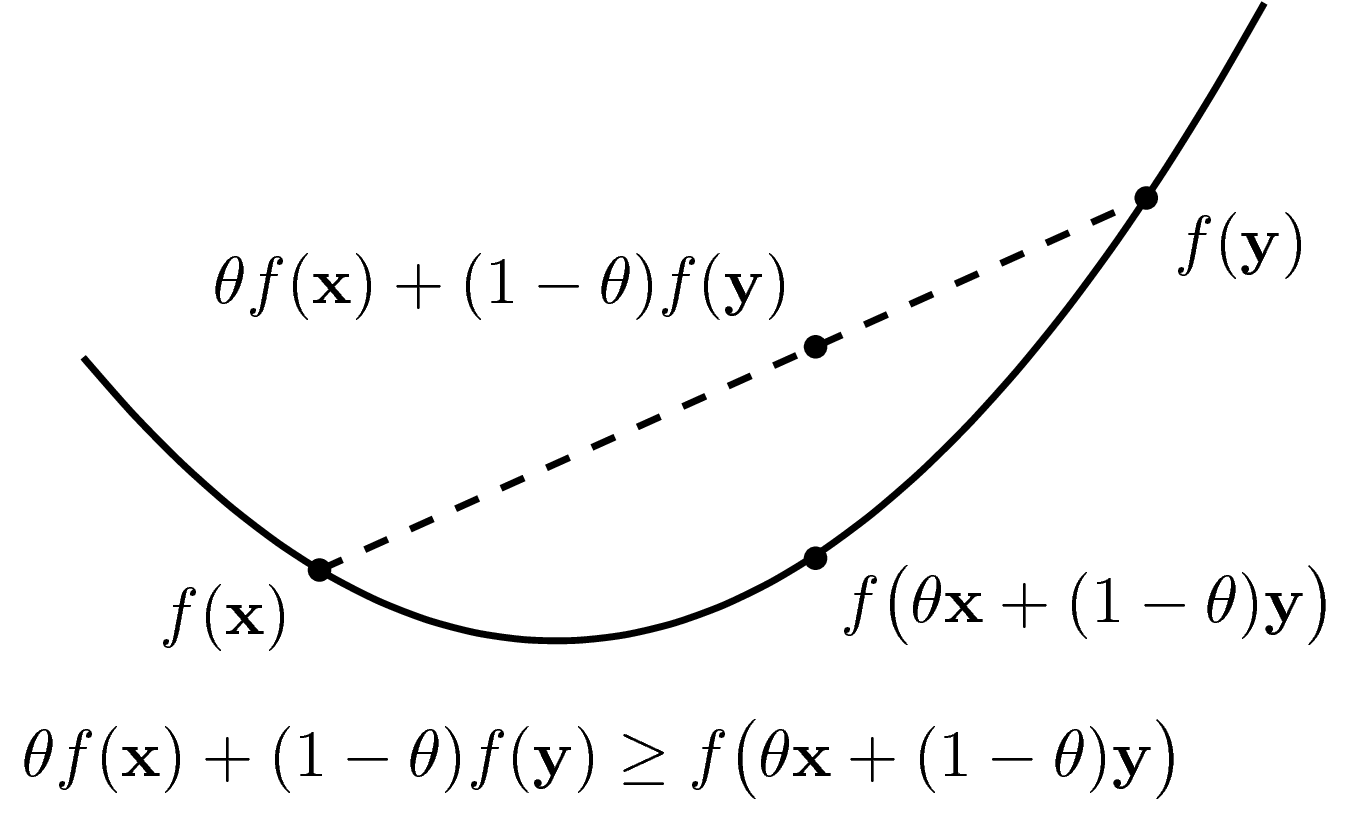
\includegraphics[width=0.6\linewidth]{Chapter2/Chapter2Figs/convexf_def}
	\caption{Hàm lồi.}
	\label{fig:hamloi}
\end{figure}

Trong khóa luận này có đề cập đến tối ưu cực đại hàm lõm. Do vậy nều $-f(x)$ là hàm lồi thì $f(x)$ là hàm lõm. Với lợi thế của bài toán có hàm mục tiêu là hàm lồi/ lõm ta luôn luôn tìm được điểm cực đại hoặc cực tiểu tốt nhất (global minimum/ maximum). Hình \ref{fig:convexnonconvex} minh họa hàm lồi và không lồi. Dễ dàng thấy được ở hàm lồi luôn chỉ có duy nhất một điểm cực tiểu ngược lại ở hàm không lồi luôn có các điểm cực tiểu địa phương và cực đại địa phương như vậy rất khó khăn hoặc bất khả thi trong việc xác định điểm cực tiểu tốt nhất cho bài toán.
\begin{figure}[H]
	\centering
	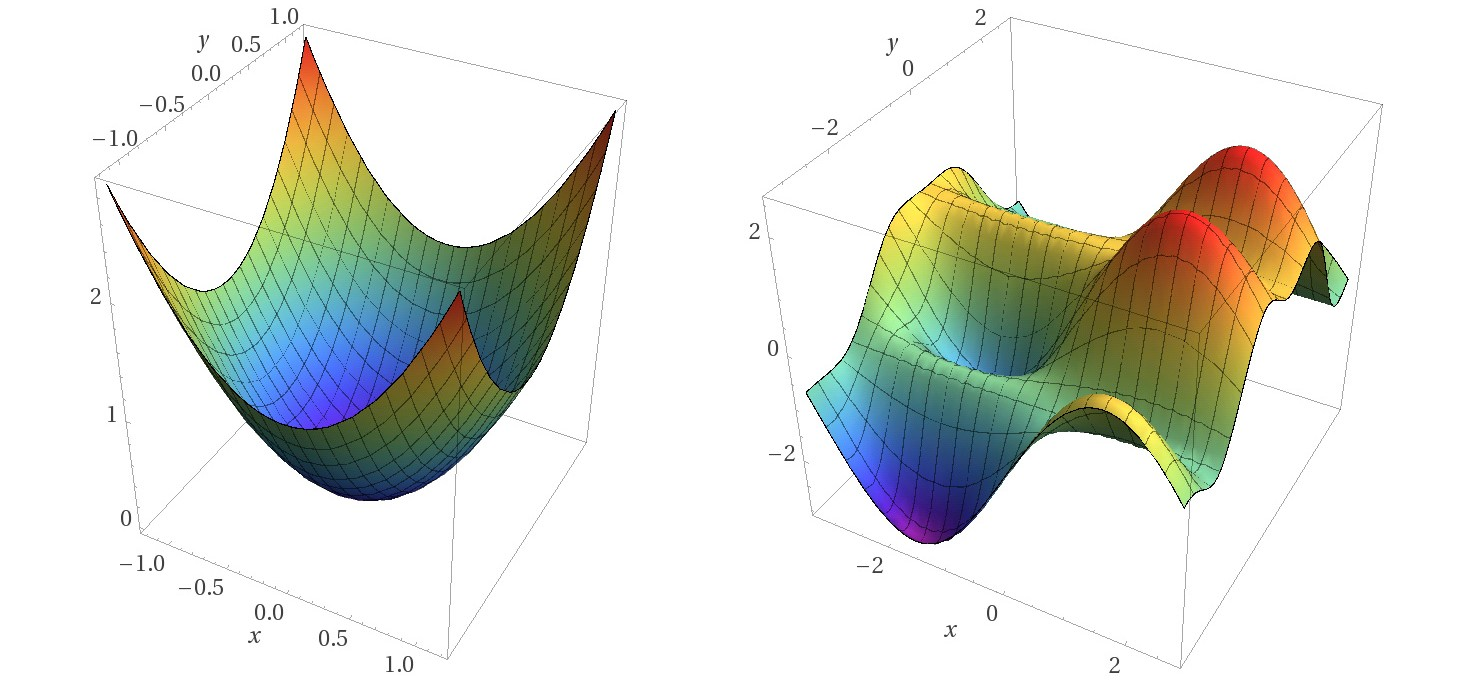
\includegraphics[width=1\linewidth]{Chapter2/Chapter2Figs/convexandnoconvex.jpg}
	\caption{Hàm lồi (trái) và hàm không lồi (phải)}
	\label{fig:convexnonconvex}
\end{figure}
\nomenclature[KN]{GD}{Gradient descent}
\nomenclature[KH]{$J(\theta)$}{Hàm chi phí}
\nomenclature[KH]{$\nabla_\theta f\left( \theta\right)$}{Đạo hàm của hàm số $f\left( \theta\right)$ theo $\theta$}
\nomenclature[KH]{$\alpha$}{Tham số tốc huấn luyện}
Một trong những phương pháp tối ưu hàm lồi được sử dụng rộng rãi cho học máy chính là phương pháp tăng\ giảm gradient nhằm ước lượng tham số $\theta$ của hô mình, khi $J(\theta)$ khả vi. Phương pháp này được trình bày trong thuật toán \ref{alg:GD} \cite{boyd2004convex} dưới đây:
\begin{algorithm}\caption{\label{alg:GD} Batch gradient descent method.}
	\begin{algorithmic}[1]
		\STATE \textbf{Given} bắt đầu từ một điểm $\theta = \{\theta_1,\dots,\theta_n\} \in \textbf{dom} f$
		\REPEAT
		\STATE 1. $\Delta \theta:=-\nabla_\theta f\left( \theta\right) $.
		\STATE 2. \text{Chọn bước nhảy $\alpha$ mặc định hoặc thông qua thuật toán backtracking line search}
		\STATE 3. \textit{Cập nhật.} $\theta:=\theta+\alpha\Delta \theta$
		\UNTIL{thuật toán hội tụ.}
	\end{algorithmic}
\end{algorithm}

Trong thuật toán \ref{alg:GD} có sử dụng phương pháp xác định $\alpha$ là tham số thể hiện bước nhảy hay tốc độ huấn luyện của thuật toán. Hình \ref{fig:learningrate} khi $\alpha$ quá lớn lớn hoặc quá nhỏ đều sẽ làm ảnh hưởng đến thời gian hội tụ của bài toán. Vì vậy trong các thuật toán giảm gradient, tốc độ học $\alpha$ cần được thay đổi phù hợp theo mỗi lần lặp. Thuật toán \ref{alg:Backtrackingls} \cite{luenberger1973introduction} được sử dụng phổ biến để xác định giá trị $\alpha$ qua mỗi lần lặp, có dễ hiểu hơn về phương pháp thông qua cách nghĩ trước nước đi trong chơi cờ.

\begin{figure}[H]
	\centering
	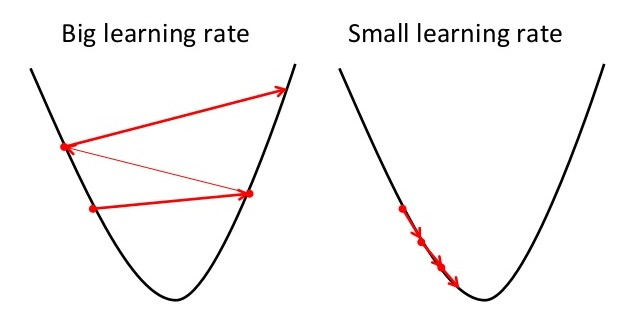
\includegraphics[width=0.8\linewidth]{Chapter2/Chapter2Figs/learningrate.jpg}
	\caption{Sự ảnh hưởng của $\alpha$ đến quá trình huấn luyện.}
	\label{fig:learningrate}
\end{figure}
\begin{algorithm}\caption{\label{alg:Backtrackingls}Backtracking line search.}
	\begin{algorithmic}
		\STATE \textbf{Given} bắt đầu tại một điểm $\bigtriangleup \theta$ với f tại $\theta \in \textbf{dom} f, \gamma \in (0,0.5), \beta \in (0,1)$
		\STATE \textbf{While} $f(\theta + \alpha\bigtriangleup \theta) > f(\theta) + \gamma\alpha\nabla f(\theta)^T \bigtriangleup \theta$ \\
		{$\alpha = \beta \alpha$}
	\end{algorithmic}
\end{algorithm}

Với hàm mục tiêu có độ phức tạp thì việc tính $\nabla f\left( x\right)$ đòi hỏi khối lượng tính toán lớn. Và nếu dữ liệu có kích thước $N$ lớn thì mỗi bước lặp có khối tượng tính toán lớn, thuật toán chạy chậm. Do vậy để tiết kiệm khối lượng tính toán, thuật toán \ref{alg:SGD} \cite{bottou2010large} phương pháp giảm gradient ngẫu nhiên là một phương pháp phù hợp trong huấn luyện dữ liệu lớn.
\nomenclature[KN]{$SGD$}{Stochastic Gradient descent}
\begin{algorithm}[H]\caption{\label{alg:SGD}Stochastic Gradient descent method.}
	\begin{algorithmic}[1]
		\STATE \textbf{Given} bắt đầu tại $\theta=\{\theta_1,\dots,\theta_n\} \in \textbf{dom} f$
		\REPEAT
		\STATE 1. Xáo trộn tập dữ liệu huấn luyện
			\FOR{ $i = 1 : N$}
				\STATE 1. $\Delta \theta:=-\nabla_\theta f\left( \theta;x^i,y^i \right) $.
				\STATE 2. \text{Chọn bước nhảy $\alpha$ mặc định hoặc thông qua thuật toán backtracking line search}
				\STATE 3. \textit{Cập nhật.} $\theta:=\theta+\alpha\Delta \theta$
			\ENDFOR
		\UNTIL{thuật toán hội tụ.}
	\end{algorithmic}
\end{algorithm}

Thuật toán \ref{alg:MBSGD} \cite{konevcny2016mini} là sự kết hợp của hai thuật toán trên phù hợp chạy trên những hệ thống tính toán song song/ phần tán được đề cập trong chương \ref{chap:c4}.
\nomenclature[KN]{$MBSGD$}{Mini-batch Stochastic Gradient descent}
\begin{algorithm}[H]\caption{\label{alg:MBSGD}Mini-batch Stochastic gradient descent method.}
	\begin{algorithmic}[1]
		\STATE \textbf{Given} bắt đầu tại $\theta=\{\theta_1,\dots,\theta_n\} \in \textbf{dom} f$ và chọn $0 \leq k \leq N$
		
		\REPEAT
		\STATE 1. xáo trộn tập dữ liệu huấn luyện
		\FOR{ $i = 1 ; i\leq N;i+=k$}
		\STATE 1. $\Delta \theta:=-\nabla_\theta f\left( \theta;x^{i:i+k},y^{i:i+k} \right) $.
		\STATE 2. \text{Chọn bước nhảy $\alpha$ mặc định hoặc thông qua thuật toán backtracking line search}
		\STATE 3. \textit{Cập nhật.} $\theta:=\theta+\alpha\Delta \theta$
		\ENDFOR
		\UNTIL{thuật toán hội tụ.}
	\end{algorithmic}
\end{algorithm}


